\chapter{Systems of Particles, Collisions, and Synoptic Mastery}
\label{ch:systems_collisions}
\begin{chapterintro}
\textbf{You will learn to:} locate the center of mass of discrete systems; apply the momentum conservation theorem to isolated systems; solve 1D and 2D elastic and inelastic collisions using the coefficient of restitution; transform between laboratory and center-of-mass frames using Koenig's theorems and reduced mass $\mu$; derive the Tsiolkovsky rocket equation; and tackle comprehensive multi-stage exam synthesis problems.
\end{chapterintro}

\section{Center of Mass and Total Momentum}

For a system of $N$ material points with masses $m_i$ and positions $\vec{r}_i$:
\begin{itemize}[leftmargin=1.4em,itemsep=3pt]
  \item The \textbf{total mass} is $M = \sum_{i=1}^N m_i$.
  \item The \textbf{center of mass} (CM) position $G$ is defined by:
        \[
        \boxed{\vec{r}_G = \frac{1}{M}\sum_{i=1}^N m_i\vec{r}_i.}
        \]
  \item The \textbf{total linear momentum} is:
        \[
        \boxed{\vec{P}_{\text{tot}} = \sum_{i=1}^N m_i\vec{v}_i = M\vec{v}_G.}
        \]
\end{itemize}

Differentiating with respect to time and separating forces into external forces $\vec{F}_{i,\text{ext}}$ and internal mutual forces $\vec{F}_{j\to i}$:
\[
\frac{\dd\vec{P}_{\text{tot}}}{\dd t} = \sum_{i=1}^N m_i\vec{a}_i = \sum_{i=1}^N \vec{F}_{i,\text{ext}} + \sum_{i=1}^N\sum_{j\ne i}^N \vec{F}_{j\to i}.
\]
By Newton's third law (action-reaction), internal forces cancel in pairs ($\vec{F}_{j\to i} + \vec{F}_{i\to j} = \vzero$).
Hence, we obtain the \textbf{Fundamental Theorem of Linear Momentum for a System}:
\[
\boxed{\frac{\dd\vec{P}_{\text{tot}}}{\dd t} = M\vec{a}_G = \sum \vec{F}_{\text{ext}}.}
\]

\begin{keyidea}[Conservation of Total Momentum]
If a system is isolated or subject to zero net external force ($\sum\vec{F}_{\text{ext}} = \vzero$):
\[
\boxed{\vec{P}_{\text{tot}} = \text{constant vector} \iff \vec{v}_G = \text{constant velocity}.}
\]
The center of mass moves in uniform rectilinear motion, completely unaffected by any internal explosions, collisions, or interactions!
\end{keyidea}

\begin{figure}[htbp]
\centering
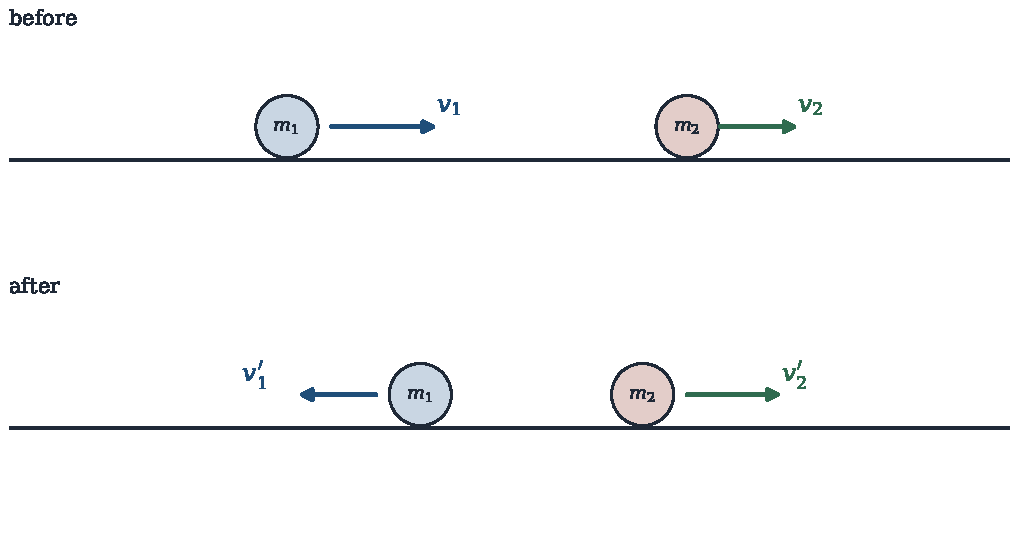
\includegraphics[width=0.72\textwidth]{figures/21_collision.pdf}
\caption{Two-particle collision in the laboratory frame. Total linear momentum $\vec{P}_{\text{tot}} = m_1\vec{v}_1 + m_2\vec{v}_2$ is conserved during the collision.}
\label{fig:collision}
\end{figure}

\section{Classification of Collisions in 1D}

In a brief collision between two bodies ($m_1, m_2$), the impact forces are so enormous that external forces (such as gravity or friction) are negligible during the collision duration $\Delta t \to 0$ (\textbf{impulsive approximation}).
Total momentum is always conserved:
\[
m_1 v_{1i} + m_2 v_{2i} = m_1 v_{1f} + m_2 v_{2f}.
\]
The elasticity of the collision is characterized by Newton's \textbf{coefficient of restitution} $e$:
\[
\boxed{e = -\frac{v_{1f} - v_{2f}}{v_{1i} - v_{2i}} = \frac{v_{\text{rel, final}}}{v_{\text{rel, initial}}} \in [0, 1].}
\]

\begin{center}
\renewcommand{\arraystretch}{1.3}
\begin{tabular}{@{}llll@{}}
\toprule
\textbf{Collision Type} & \textbf{Restitution $e$} & \textbf{Kinetic Energy $\Delta E_c$} & \textbf{Outcome} \\
\midrule
\textbf{Perfectly Elastic} & $e = 1$ & $\Delta E_c = 0$ (conserved) & $v_{1f} - v_{2f} = -(v_{1i} - v_{2i})$ \\
\textbf{Inelastic} & $0 < e < 1$ & $\Delta E_c < 0$ (partially lost) & Bodies bounce apart with reduced relative speed \\
\textbf{Perfectly Inelastic} & $e = 0$ & Maximum energy loss & Bodies stick together: $v_{1f} = v_{2f} = v_G$ \\
\bottomrule
\end{tabular}
\end{center}

For a 1D collision with known $e$, the final velocities are uniquely determined:
\[
\boxed{v_{1f} = v_G - \frac{m_2}{m_1 + m_2}e(v_{1i} - v_{2i}), \qquad v_{2f} = v_G + \frac{m_1}{m_1 + m_2}e(v_{1i} - v_{2i}).}
\]

\section{Center-of-Mass Frame and Koenig's First Theorem}

Let $\mathcal{R}^*$ be the center-of-mass frame (translating with velocity $\vec{v}_G$).
In this frame, the total linear momentum is identically zero: $\vec{P}^* = \vzero$.
The velocities in the laboratory and CM frames are related by $\vec{v}_i = \vec{v}_G + \vec{v}_i^*$.
The total kinetic energy in the laboratory frame satisfies \textbf{Koenig's First Theorem}:
\[
\boxed{E_c = \frac{1}{2}M v_G^2 + E_c^*,}
\]
where for a two-body system, the internal kinetic energy in the CM frame simplifies to:
\[
\boxed{E_c^* = \frac{1}{2}\mu\,v_{\text{rel}}^2, \quad \text{with reduced mass } \mu = \frac{m_1 m_2}{m_1 + m_2}.}
\]
In a collision, the kinetic energy of the center of mass $\frac{1}{2}M v_G^2$ can never be lost because $\vec{v}_G$ is constant!
The maximum possible kinetic energy that can be converted into heat/deformation (in a totally inelastic collision) is precisely $E_c^* = \frac{1}{2}\mu v_{\text{rel}}^2$.

\section{Worked Examples}

\begin{worked}[The ballistic pendulum]
A wooden block of mass $M = 1.98\ \mathrm{kg}$ hangs from light strings of length $L = 1.50\ \mathrm{m}$. A bullet of mass $m = 20.0\ \mathrm{g} = 0.0200\ \mathrm{kg}$ is fired horizontally into the block and embeds itself inside it. After impact, the block and bullet swing upward together to a maximum height $h = 8.50\ \mathrm{cm} = 0.0850\ \mathrm{m}$.
Find the initial speed $v_0$ of the bullet and the mechanical energy lost in the collision.
\end{worked}

\begin{solution}{16.1}
The problem consists of two distinct stages:
\begin{enumerate}[leftmargin=1.5em,itemsep=2pt]
  \item \textbf{Stage 1: Inelastic impact (duration $\Delta t \to 0$)}.
  External forces (gravity and string tension) do not have time to act horizontally. Total horizontal momentum is conserved:
  \[
  m v_0 = (M + m) V \implies V = \frac{m}{M + m}v_0,
  \]
  where $V$ is the speed of the combined mass immediately after impact.
  \item \textbf{Stage 2: Conservative upward swing}.
  After the collision, the tension in the strings does no work ($\vec{T}\perp\vec{v}$), and only gravity acts. Mechanical energy is conserved:
  \[
  \frac{1}{2}(M + m)V^2 = (M + m)gh \implies V = \sqrt{2gh}.
  \]
\end{enumerate}
Equating the two expressions for $V$:
\[
\frac{m}{M + m}v_0 = \sqrt{2gh} \implies \boxed{v_0 = \frac{M + m}{m}\sqrt{2gh}.}
\]
Computing numerically:
\[
\sqrt{2gh} = \sqrt{2(9.81)(0.0850)} = \sqrt{1.6677} \approx 1.291\ \mathrm{m\,s^{-1}}.
\]
Mass ratio: $\frac{M + m}{m} = \frac{1.98 + 0.0200}{0.0200} = \frac{2.00}{0.0200} = 100$.
The initial bullet speed is:
\[
v_0 = 100\times 1.291 = \mathbf{129.1\ \mathrm{m\,s^{-1}}.}
\]
Energy loss:
\begin{align*}
E_{c,\text{initial}} &= \frac{1}{2}m v_0^2 = \frac{1}{2}(0.0200)(129.1)^2 \approx 166.7\ \mathrm{J}, \\
E_{c,\text{after impact}} &= \frac{1}{2}(M + m)V^2 = \frac{1}{2}(2.00)(1.291)^2 \approx 1.67\ \mathrm{J}.
\end{align*}
The fraction of energy retained is only $\frac{m}{M+m} = \frac{1}{100} = 1\%$.
The mechanical energy lost is $\Delta E = 166.7 - 1.67 = \mathbf{165.0\ \mathrm{J}}$ ($99\%$ converted into heat, sound, and plastic deformation of the wood).
\end{solution}

\begin{worked}[Glancing 2D elastic collision of equal masses]
In a nuclear physics experiment, a proton of mass $m$ moving with speed $v_0$ collides elastically with another proton of equal mass $m$ initially at rest.
Prove that after the collision, the two protons always fly apart at a right angle ($90^\circ$), provided the collision is not head-on.
\end{worked}

\begin{solution}{16.2}
Let $\vec{v}_1$ and $\vec{v}_2$ be the final velocity vectors of the two protons after the collision.
\begin{itemize}[leftmargin=1.4em,itemsep=2pt]
  \item Conservation of linear momentum:
        \[
        m\vec{v}_0 = m\vec{v}_1 + m\vec{v}_2 \implies \vec{v}_0 = \vec{v}_1 + \vec{v}_2.
        \]
  \item Conservation of kinetic energy (elastic collision):
        \[
        \frac{1}{2}m v_0^2 = \frac{1}{2}m v_1^2 + \frac{1}{2}m v_2^2 \implies v_0^2 = v_1^2 + v_2^2.
        \]
\end{itemize}
Now take the dot product of the momentum vector equation with itself:
\[
\vec{v}_0\cdot\vec{v}_0 = (\vec{v}_1 + \vec{v}_2)\cdot(\vec{v}_1 + \vec{v}_2) \implies v_0^2 = v_1^2 + v_2^2 + 2\,\vec{v}_1\cdot\vec{v}_2.
\]
Subtracting the energy conservation equation ($v_0^2 = v_1^2 + v_2^2$):
\[
0 = 2\,\vec{v}_1\cdot\vec{v}_2 \implies \boxed{\vec{v}_1\cdot\vec{v}_2 = 0.}
\]
Since neither proton is at rest ($\vec{v}_1\ne\vzero, \vec{v}_2\ne\vzero$), their final velocity vectors are strictly orthogonal:
\[
\theta_1 + \theta_2 = \mathbf{90.0^\circ.}
\]
This iconic result is routinely observed in bubble chamber and cloud chamber photographs of proton-proton collisions.
\end{solution}

\section{Exercises and Step-by-Step Solutions}

\begin{exercise}{\warm\ Center of mass of a three-particle system}
Three masses lie in the $xy$-plane: $m_1 = 1.00\ \mathrm{kg}$ at $(1.0, 2.0)\ \mathrm{m}$, $m_2 = 2.00\ \mathrm{kg}$ at $(4.0, 1.0)\ \mathrm{m}$, and $m_3 = 3.00\ \mathrm{kg}$ at $(2.0, 5.0)\ \mathrm{m}$.
(a) Calculate the coordinates $(x_G, y_G)$ of the center of mass.
(b) If particle $m_1$ moves with velocity $\vec{v}_1 = 6.0\,\ihat\ \mathrm{m\,s^{-1}}$ while $m_2$ and $m_3$ are stationary, find the velocity $\vec{v}_G$ of the center of mass.
\end{exercise}

\begin{tabletworkspace}[5.0cm]
\end{tabletworkspace}

\begin{solution}{16.1}
(a) Total mass: $M = m_1 + m_2 + m_3 = 1.00 + 2.00 + 3.00 = 6.00\ \mathrm{kg}$.
Center of mass coordinates:
\begin{align*}
x_G &= \frac{m_1 x_1 + m_2 x_2 + m_3 x_3}{M} = \frac{1.00(1.0) + 2.00(4.0) + 3.00(2.0)}{6.00} = \frac{1.0 + 8.0 + 6.0}{6.00} = \frac{15.0}{6.00} = \mathbf{2.50\ \mathrm{m}.} \\
y_G &= \frac{m_1 y_1 + m_2 y_2 + m_3 y_3}{M} = \frac{1.00(2.0) + 2.00(1.0) + 3.00(5.0)}{6.00} = \frac{2.0 + 2.0 + 15.0}{6.00} = \frac{19.0}{6.00} \approx \mathbf{3.17\ \mathrm{m}.}
\end{align*}
Thus $\vec{r}_G = 2.50\,\ihat + 3.17\,\jhat\ \mathrm{m}$.

(b) Total linear momentum:
\[
\vec{P}_{\text{tot}} = m_1\vec{v}_1 + m_2\vec{v}_2 + m_3\vec{v}_3 = (1.00)(6.0\,\ihat) + \vzero + \vzero = 6.0\,\ihat\ \mathrm{kg\,m\,s^{-1}}.
\]
The center of mass velocity is:
\[
\vec{v}_G = \frac{\vec{P}_{\text{tot}}}{M} = \frac{6.0\,\ihat}{6.00} = \mathbf{1.00\,\ihat\ \mathrm{m\,s^{-1}}.}
\]
\end{solution}

\begin{exercise}{\warm\ 1D elastic collision and neutron moderation}
In a nuclear reactor, fast fission neutrons of mass $m_1 \approx 1\ \mathrm{u}$ moving at initial speed $v_0$ must be slowed down by head-on elastic collisions with stationary moderator nuclei of mass $m_2$.
(a) For a head-on elastic collision with $m_2$ at rest, show that the final speed of the neutron is:
\[
v_{1f} = \frac{m_1 - m_2}{m_1 + m_2}v_0.
\]
(b) Show that the fraction of kinetic energy transferred to the moderator nucleus is:
\[
\frac{\Delta E_c}{E_{c0}} = \frac{4 m_1 m_2}{(m_1 + m_2)^2}.
\]
(c) Evaluate this energy transfer fraction for a collision with ordinary hydrogen ($m_2 = 1\ \mathrm{u}$), carbon ($m_2 = 12\ \mathrm{u}$), and lead ($m_2 = 207\ \mathrm{u}$). Explain why water is an excellent neutron moderator while heavy metals are ineffective.
\end{exercise}

\begin{tabletworkspace}[5.5cm]
\end{tabletworkspace}

\begin{solution}{16.2}
(a) For an elastic collision ($e = 1$) with $v_{2i} = 0$:
\[
\text{Momentum:}\quad m_1 v_0 = m_1 v_{1f} + m_2 v_{2f}, \qquad \text{Restitution:}\quad v_{2f} - v_{1f} = v_0 \implies v_{2f} = v_0 + v_{1f}.
\]
Substituting into the momentum equation:
\[
m_1 v_0 = m_1 v_{1f} + m_2(v_0 + v_{1f}) = (m_1 + m_2)v_{1f} + m_2 v_0.
\]
Rearranging:
\[
(m_1 - m_2)v_0 = (m_1 + m_2)v_{1f} \implies \boxed{v_{1f} = \frac{m_1 - m_2}{m_1 + m_2}v_0.}
\]

(b) The final kinetic energy of the neutron is:
\[
E_{c1,f} = \frac{1}{2}m_1 v_{1f}^2 = \frac{1}{2}m_1 v_0^2\left(\frac{m_1 - m_2}{m_1 + m_2}\right)^2 = E_{c0}\left(\frac{m_1 - m_2}{m_1 + m_2}\right)^2.
\]
The kinetic energy transferred to the moderator nucleus is:
\[
\frac{\Delta E_c}{E_{c0}} = 1 - \left(\frac{m_1 - m_2}{m_1 + m_2}\right)^2 = \frac{(m_1 + m_2)^2 - (m_1 - m_2)^2}{(m_1 + m_2)^2} = \boxed{\frac{4m_1 m_2}{(m_1 + m_2)^2}.}
\]

(c) Numerical evaluation:
\begin{itemize}[leftmargin=1.4em,itemsep=2pt]
  \item Hydrogen ($m_2 = 1\ \mathrm{u}$): $\frac{4(1)(1)}{(1+1)^2} = \frac{4}{4} = \mathbf{1.00 = 100\%.}$ In a head-on collision with a proton, the neutron transfers $100\%$ of its kinetic energy and stops completely!
  \item Carbon-12 ($m_2 = 12\ \mathrm{u}$): $\frac{4(1)(12)}{(1+12)^2} = \frac{48}{169} \approx \mathbf{0.284 = 28.4\%.}$
  \item Lead-207 ($m_2 = 207\ \mathrm{u}$): $\frac{4(1)(207)}{(1+207)^2} = \frac{828}{(208)^2} = \frac{828}{43264} \approx \mathbf{0.019 = 1.9\%.}$
\end{itemize}
Because hydrogen nuclei (protons) match the neutron mass almost exactly, water ($\mathrm{H_2O}$) slows down neutrons rapidly in very few collisions. Heavy nuclei like lead barely recoil, bouncing the neutron elastically with almost zero energy loss!
\end{solution}

\begin{exercise}{\core\ Bouncing ball with coefficient of restitution $e$}
A rubber ball is dropped from rest from an initial height $h_0$ onto a rigid horizontal floor. The collision has a constant coefficient of restitution $e \in (0, 1)$.
(a) Find the height $h_n$ reached after the $n$-th bounce.
(b) Find the time interval $t_n$ between the $(n-1)$-th bounce and the $n$-th bounce.
(c) Sum the infinite geometric series to compute the total time $T_{\text{total}}$ until the ball stops bouncing, and the total distance $D_{\text{total}}$ traveled.
\end{exercise}

\begin{tabletworkspace}[6.0cm]
\end{tabletworkspace}

\begin{solution}{16.3}
(a) The impact speed before the first bounce is $v_1 = \sqrt{2gh_0}$.
After rebound, its speed is $u_1 = e v_1$.
The height reached after the first rebound is $h_1 = \frac{u_1^2}{2g} = \frac{e^2 v_1^2}{2g} = e^2 h_0$.
By induction, after $n$ rebounds:
\[
\boxed{h_n = e^{2n}h_0.}
\]

(b) Time to fall from $h_0$ to the first bounce: $t_0 = \sqrt{\frac{2h_0}{g}}$.
For each subsequent bounce $n \ge 1$, the ball goes up to height $h_n$ and falls back down, so the time between bounces is:
\[
t_n = 2\sqrt{\frac{2h_n}{g}} = 2\sqrt{\frac{2(e^{2n}h_0)}{g}} = 2e^n\sqrt{\frac{2h_0}{g}} = 2e^n t_0.
\]

(c) Total time to stop bouncing:
\[
T_{\text{total}} = t_0 + \sum_{n=1}^\infty t_n = t_0 + 2t_0\sum_{n=1}^\infty e^n = t_0\left( 1 + 2\frac{e}{1 - e} \right) = t_0\left(\frac{1 - e + 2e}{1 - e}\right) = \boxed{\sqrt{\frac{2h_0}{g}}\left(\frac{1 + e}{1 - e}\right).}
\]
Remarkably, although the ball undergoes infinitely many bounces, the total time is \textbf{finite}!

Total distance traveled:
\[
D_{\text{total}} = h_0 + 2\sum_{n=1}^\infty h_n = h_0 + 2h_0\sum_{n=1}^\infty e^{2n} = h_0\left( 1 + \frac{2e^2}{1 - e^2} \right) = \boxed{h_0\left(\frac{1 + e^2}{1 - e^2}\right).}
\]
\end{solution}

\begin{exercise}{\core\ The Tsiolkovsky Rocket Equation}
A rocket of total initial mass $m_0$ in deep space (zero gravity and zero drag) accelerates by ejecting burned propellant backward at a constant speed $u_{\text{ex}}$ relative to the rocket.
(a) In an inertial frame where the rocket has velocity $v$, analyze the momentum balance between time $t$ and $t + \dd t$ when mass $-\dd m$ ($\dd m < 0$) is ejected at speed $v - u_{\text{ex}}$ to derive the differential equation:
\[
m\,\dd v = -u_{\text{ex}}\,\dd m.
\]
(b) Integrate this equation to derive the famous \textbf{Tsiolkovsky Rocket Equation}:
\[
\Delta v = v_f - v_0 = u_{\text{ex}}\ln\left(\frac{m_0}{m_f}\right).
\]
(c) A rocket has an exhaust velocity $u_{\text{ex}} = 3000\ \mathrm{m\,s^{-1}}$. What mass ratio $m_0/m_f$ is required to achieve Earth orbital velocity $\Delta v = 7.80\ \mathrm{km\,s^{-1}}$?
\end{exercise}

\begin{tabletworkspace}[5.5cm]
\end{tabletworkspace}

\begin{solution}{16.4}
(a) At time $t$: the rocket and remaining fuel have mass $m$ and velocity $v$.
The total momentum is:
\[
P(t) = mv.
\]
At time $t + \dd t$: fuel of mass $\dd m_{\text{fuel}} = -\dd m > 0$ has been expelled backward with velocity $v - u_{\text{ex}}$ relative to the inertial frame. The rocket has mass $m + \dd m$ and velocity $v + \dd v$.
The momentum is:
\[
P(t + \dd t) = (m + \dd m)(v + \dd v) + (-\dd m)(v - u_{\text{ex}}) = mv + m\,\dd v + v\,\dd m + \dd m\dd v - v\,\dd m + u_{\text{ex}}\,\dd m.
\]
Dropping the second-order differential $\dd m\dd v$:
\[
P(t + \dd t) = mv + m\,\dd v + u_{\text{ex}}\,\dd m.
\]
Since no external force acts ($F_{\text{ext}} = 0$):
\[
P(t + \dd t) - P(t) = 0 \implies m\,\dd v + u_{\text{ex}}\,\dd m = 0 \implies \boxed{m\,\dd v = -u_{\text{ex}}\,\dd m.}
\]

(b) Dividing by $m$:
\[
\dd v = -u_{\text{ex}}\frac{\dd m}{m}.
\]
Integrating from initial state $(m_0, v_0)$ to final empty propellant burnout state $(m_f, v_f)$:
\[
\int_{v_0}^{v_f} \dd v = -u_{\text{ex}}\int_{m_0}^{m_f} \frac{\dd m}{m} \implies v_f - v_0 = -u_{\text{ex}}\left[ \ln m_f - \ln m_0 \right].
\]
Using $\ln(m_f/m_0) = -\ln(m_0/m_f)$:
\[
\boxed{\Delta v = u_{\text{ex}}\ln\left(\frac{m_0}{m_f}\right).}
\]

(c) Given $\Delta v = 7800\ \mathrm{m\,s^{-1}}$ and $u_{\text{ex}} = 3000\ \mathrm{m\,s^{-1}}$:
\[
\ln\left(\frac{m_0}{m_f}\right) = \frac{\Delta v}{u_{\text{ex}}} = \frac{7800}{3000} = 2.60.
\]
Taking the exponential:
\[
\frac{m_0}{m_f} = e^{2.60} \approx \mathbf{13.46.}
\]
This means the fuel must constitute $\frac{13.46 - 1}{13.46} \approx \mathbf{92.6\%}$ of the rocket's total launch mass! This exponential dependence explains why multi-stage rockets are essential for space exploration.
\end{solution}

\begin{exercise}{\mastery\ Synoptic Problem: The Spring Launcher and Vertical Loop}
A block of mass $m=0.500\ \mathrm{kg}$ is pushed against a horizontal spring of stiffness $k=800\ \mathrm{N\,m^{-1}}$, compressing it by $\Delta x = 0.200\ \mathrm{m}$.
Upon release, the block moves along a smooth horizontal track, crosses a rough horizontal patch of length $d=0.800\ \mathrm{m}$ with kinetic friction coefficient $\mu_k = 0.250$, and then enters a smooth vertical circular loop of radius $R = 0.500\ \mathrm{m}$.
(a) Find the speed $v_1$ of the block immediately after separating from the spring.
(b) Find the speed $v_2$ after traversing the rough patch.
(c) Determine whether the block completes the loop without falling off, and calculate the normal reaction force $N_{\text{top}}$ at the very top of the loop.
\end{exercise}

\begin{tabletworkspace}[6.5cm]
\end{tabletworkspace}

\begin{solution}{16.5}
(a) From release to spring separation: only the conservative spring force acts.
Mechanical energy conservation:
\[
E_{m0} = \frac{1}{2}k(\Delta x)^2 = \frac{1}{2}m v_1^2 \implies v_1 = \Delta x\sqrt{\frac{k}{m}}.
\]
Computing:
\[
v_1 = 0.200\sqrt{\frac{800}{0.500}} = 0.200\sqrt{1600} = 0.200\times 40.0 = \mathbf{8.00\ \mathrm{m\,s^{-1}}.}
\]

(b) Across the rough patch of length $d$: friction does work $W_f = -\mu_k mg d$.
Work-energy theorem:
\[
\frac{1}{2}m v_2^2 - \frac{1}{2}m v_1^2 = -\mu_k mg d \implies v_2^2 = v_1^2 - 2\mu_k gd.
\]
Computing:
\[
v_2^2 = (8.00)^2 - 2(0.250)(9.81)(0.800) = 64.0 - 3.924 = 60.076\ \mathrm{m^2\,s^{-2}}.
\]
\[
v_2 = \sqrt{60.076} \approx \mathbf{7.75\ \mathrm{m\,s^{-1}}.}
\]

(c) In the smooth vertical loop: only gravity performs work as the block rises to height $2R = 2(0.500) = 1.00\ \mathrm{m}$.
Work-energy theorem to the top of the loop:
\[
\frac{1}{2}m v_{\text{top}}^2 - \frac{1}{2}m v_2^2 = -mg(2R) \implies v_{\text{top}}^2 = v_2^2 - 4gR.
\]
Computing:
\[
v_{\text{top}}^2 = 60.076 - 4(9.81)(0.500) = 60.076 - 19.62 = 40.456\ \mathrm{m^2\,s^{-2}} \implies v_{\text{top}} \approx 6.36\ \mathrm{m\,s^{-1}}.
\]
The condition to complete the loop without leaving the track is $v_{\text{top}}^2 \ge gR$:
\[
gR = 9.81\times 0.500 = 4.905\ \mathrm{m^2\,s^{-2}}.
\]
Since $v_{\text{top}}^2 = 40.46 \gg 4.91$, the block \textbf{comfortably completes the loop}!
The normal force at the top is:
\[
N_{\text{top}} = m\frac{v_{\text{top}}^2}{R} - mg = \frac{0.500\times 40.456}{0.500} - 0.500(9.81) = 40.456 - 4.905 \approx \mathbf{35.55\ \mathrm{N}.}
\]
\end{solution}

\begin{exercise}{\mastery\ Synoptic Problem: Gravitational Slingshot (Planetary Flyby)}
A spacecraft of mass $m$ approaches Jupiter (mass $M \gg m$) which orbits the Sun at speed $V_J = 13.0\ \mathrm{km\,s^{-1}}$. In the solar frame, the spacecraft moves with speed $v_0 = 10.0\ \mathrm{km\,s^{-1}}$ directly toward Jupiter (head-on encounter).
(a) Using a Galilean transformation, find the velocity $u_i$ of the spacecraft in Jupiter's rest frame before the encounter.
(b) Since gravitational deflection is an elastic scattering in Jupiter's rest frame, the spacecraft swings around Jupiter and emerges traveling in the opposite direction. What is its speed $u_f$ in Jupiter's frame?
(c) Transform back to the solar frame to find the final speed $v_f$ of the spacecraft. How much kinetic energy did the spacecraft gain from Jupiter's orbital motion?
\end{exercise}

\begin{tabletworkspace}[6.0cm]
\end{tabletworkspace}

\begin{solution}{16.6}
(a) Choose the $x$-axis in the direction of Jupiter's orbital motion: $\vec{V}_J = +V_J\ihat = +13.0\,\ihat\ \mathrm{km\,s^{-1}}$.
The incoming spacecraft travels toward Jupiter in head-on approach: $\vec{v}_0 = -v_0\ihat = -10.0\,\ihat\ \mathrm{km\,s^{-1}}$.
In Jupiter's reference frame $\mathcal{R}_J$, the relative velocity is:
\[
\vec{u}_i = \vec{v}_0 - \vec{V}_J = -10.0\,\ihat - 13.0\,\ihat = \mathbf{-23.0\,\ihat\ \mathrm{km\,s^{-1}}.}
\]
The spacecraft approaches Jupiter at speed $u_i = 23.0\ \mathrm{km\,s^{-1}}$.

(b) In Jupiter's frame, the spacecraft moves in a conservative gravitational hyperbola. By conservation of energy in $\mathcal{R}_J$, the outgoing asymptotic speed equals the incoming asymptotic speed:
\[
u_f = u_i = 23.0\ \mathrm{km\,s^{-1}}.
\]
After completing a $180^\circ$ swing around the planet, its outgoing velocity in Jupiter's frame is reversed:
\[
\vec{u}_f = +u_i\ihat = \mathbf{+23.0\,\ihat\ \mathrm{km\,s^{-1}}.}
\]

(c) Transforming back to the Sun's inertial frame:
\[
\vec{v}_f = \vec{u}_f + \vec{V}_J = +23.0\,\ihat + 13.0\,\ihat = \mathbf{+36.0\,\ihat\ \mathrm{km\,s^{-1}}.}
\]
The final speed is:
\[
\boxed{v_f = v_0 + 2V_J = 10.0 + 2(13.0) = \mathbf{36.0\ \mathrm{km\,s^{-1}}!}}
\]
The spacecraft has gained $\Delta v = 26.0\ \mathrm{km\,s^{-1}}$!
Kinetic energy change per unit mass:
\[
\Delta\left(\frac{E_c}{m}\right) = \frac{1}{2}v_f^2 - \frac{1}{2}v_0^2 = \frac{1}{2}(36.0^2 - 10.0^2) = \frac{1}{2}(1296 - 100) = \mathbf{598\ \mathrm{MJ\,kg^{-1}}.}
\]
This tremendous energy boost is taken directly from Jupiter's enormous orbital kinetic energy around the Sun (slowing Jupiter down by an utterly imperceptible $\Delta V_J \sim 10^{-21}\ \mathrm{m\,s^{-1}}$). This is the gravity assist technique used by the Voyager, Cassini, and New Horizons probes!
\end{solution}
